\chapter{CÂY DFS (DEPTH-FIRST SEARCH TREE) VÀ ỨNG DỤNG}

\minitoc

\section{Nguồn tài nguyên}
Nội dung bài chủ yếu tham khảo/copy từ [VNOI WIKI]: \url{https://wiki.vnoi.info/algo/graph-theory/Depth-First-Search-Tree.md}

\section{Khái niệm cây duyệt chiều sâu DFS (cây DFS)}

Trong quá trình $DFS$, với mỗi đỉnh $u$ ta có $par[u]$ là số hiệu của đỉnh mà từ đỉnh đó thủ tục $DFS$ gọi để quy đến $u$. Xây dựng đồ thị con với các cạnh là $(par[u], u)$, ta có được một cây. Cây này được gọi là \textbf{cây $DFS$}.   

Các cạnh thuộc cây $DFS$ được gọi là các ``cạnh nét liền''.

Các cạnh còn lại không thuộc cây $DFS$ được gọi là các ``cạnh nét đứt''.\\

Nói cách khác, khi ta thực hiện $DFS$, tưởng tượng như sau:

\begin{enumerate}
    \item Bắt đầu từ một đỉnh gốc:

    – Ta gọi DFS tại đó, coi nó là “gốc” của cây.
    \item Mỗi lần đi từ u xuống v lần đầu tiên
    
    – Nếu v chưa được thăm, ta đánh dấu par[v] = u (vì u ``gọi'' v), và gọi tiếp DFS(v).
    
    – Cạnh (u, v) đó chính là một cạnh cây (nét liền), vì nó nằm trên hành trình ta thực sự đi.
    \item Khi gặp một cạnh nối u với một đỉnh v đã thăm rồi
    
    – Ta không đi tiếp, vì v đã vào cây.

    – Cạnh đó được gọi là cạnh không phải cây (nét đứt). Nó chỉ là ``đường tắt'' giữa hai đỉnh đã có trong cây.
\end{enumerate}


\begin{figure}[h]
    \centering
    \includegraphics[width=0.3\textwidth]{resource/img/b3/Depth-First-Search-Tree_img1.png}
    \caption{Minh họa cây DFS}    
\end{figure}

Trong đồ thị có hướng, xét các cung được thăm và không được thăm bởi $DFS$, ta có 4 loại cung sau:
\begin{itemize}
    \item Cung của cây $DFS$ \textbf{(Tree egde):} là các cung thuộc cây $DFS$ được định hướng theo chiều từ cha đến con. (ví dụ cạnh $(u, v)$ thuộc cây $DFS$ mà $u$ được thăm trước $v$ hay $u$ là cha của $v$ thì ta có cung $u \rightarrow v$ là cung của cây $DFS$). < Các cung của cây $DFS$ được đánh dấu là các cạnh màu đen trong hình bên dưới >
    \item Cung xuôi \textbf{(Forward edge):} là các cung không thuộc cây $DFS$ và có dạng $u \rightarrow v$ trong đó $u$ là tổ tiên của $v$ trong cây $DFS$. < Các cung xuôi được đánh dấu là các cạnh màu xanh lá trong hình bên dưới >
    \item Cung ngược \textbf{(Back edge):} là các cung không thuộc cây $DFS$ và có dạng $v \rightarrow u$ trong đó $u$ là tổ tiên của $v$ trong cây $DFS$. < Các cung ngược được đánh dấu là các cạnh màu đỏ trong hình bên dưới >
    \item Cung chéo \textbf{(Cross edge):} là các cung không thuộc cây $DFS$ và có dạng $u \rightarrow v$ trong đó $u$ và $v$ thuộc hai nhánh khác nhau của cùng một cây $DFS$. < Các cung chéo được đánh dấu là các cạnh màu xanh dương trong hình bên dưới >
\end{itemize}

\begin{figure}[h]
    \centering
    \includegraphics[width=0.2\textwidth]{resource/img/b3/Depth-First-Search-Tree_img2.png}   
    \caption{Mô tả các loại cung trong cây} 
\end{figure}


Trong đồ thị vô hướng:
\begin{itemize}
    \item Không tồn tại cung chéo. Vì khi đỉnh $u$ được duyệt trong hàm $DFS$ ta sẽ duyệt tất cả các đỉnh $v$ kề $u$ mà $v$ chưa được thăm. Như vậy nếu tồn tại một cung chéo $(u, v)$ chứng tỏ khi duyệt đến đỉnh $u$ hoặc đỉnh $v$ ta đã không duyệt cạnh $(u, v)$.
    \item Vì các cạnh trên đồ thị vô hướng không được định chiều nên không thể định nghĩa 2 loại cung xuôi và cung ngược như ở đồ thị có hướng. Do đó, ở đồ thị vô hướng, cung xuôi và cung ngược sẽ được định nghĩa như sau:
    \begin{itemize}
        \item Cung xuôi \textbf{(Forward edge):} là các cung thuộc cây $DFS$. Hay còn có cách gọi khác là ``cạnh nét liền'' hoặc ``cung của cây $DFS$''.
        \item Cung ngược (Back edge): là các cung không thuộc cây $DFS$. Hay còn có cách gọi khác là ``cạnh nét đứt''.
    \end{itemize}
    \item Như vậy trên đồ thị vô hướng lúc này chỉ còn  loại cung là cung ngược và cung xuôi (cung của cây $DFS$).
\end{itemize}

\textbf{Một số mảng quan trọng trong cây DFS:}

\begin{itemize}
    \item Mảng \textbf{num[]}: cho biết thứ tự duyệt DFS của các đỉnh (thứ tự mà mỗi đỉnh bắt đầu duyệt).
    \item Mảng \textbf{low[]}: Với mỗi đỉnh $u$, $low[u]$ cho biết thứ tự (giá trị $num$) nhỏ nhất có thể đi đến được từ $u$ bằng cách đi xuôi xuống theo các cạnh nét liền (các cung trên cây DFS) và kết thúc đi ngược lên không quá 1 lần theo cạnh nét đứt. Ngoài ra ta cũng có thể hiểu ý nghĩa của $low[u]$ là thứ tự thăm của đỉnh có thứ tự thăm sớm nhất nằm trong cây con gốc $u$ hoặc kề cạnh với 1 đỉnh bất kì nằm trong cây con gốc $u$.
    \item Mảng \textbf{tail[]}: cho biết thời điểm kết thúc duyệt DFS của mỗi đỉnh cũng là thời điểm duyệt xong của đỉnh đó.
\end{itemize}

\noindent\textbf{Nhận xét:} Các đỉnh có thứ tự thăm nằm trong khoảng từ $num[u]$ đến $tail[u]$ chính là các đỉnh nằm trong cây con gốc $u$ trong cây DFS.\\

\textbf{Cách tính mảng low[], num[], tail[]:}

\begin{itemize}
    \item \textbf{Ý tưởng chính:} Mảng $num[]$, $tail[]$ ta có thể tính dễ dàng bằng cách DFS xác định thời điểm duyệt tới và thời điểm duyệt xong của các đỉnh. Với mảng $low[]$ ta có:
    \begin{itemize}
        \item Trước hết, với 1 đỉnh $u$ bất kì có thể tự đi tới chính nó nên ta gán $low[u] = num[u]$.
        \item Từ $u$ có thể đến các đỉnh $v$ kề u bằng 1 cạnh nét đứt nên ta có $low[u] = \min(low[u], num[v])$ với $(u, v)$ là một cạnh nét đứt.
        \item Ngược lại, nếu $(u, v)$ là một cạnh nét liền và v không phải cha của u ta có $low[u] = \min(low[u], low[v])$ do từ $u$ ta có thể đi xuống $v$ sau đó đi theo con đường đã xác định ở đỉnh $v$ để tới đỉnh có thứ tự thăm là $low[v]$.
    \end{itemize}
    \item \textbf{Chú ý:} Giá trị thực sự của $num[], low[]$ được xác định bằng giá trị thực sự của $low[u], tail[u]$ chỉ được xác định khi đã duyệt xong đỉnh $u$. Thời điểm duyệt tới của một đỉnh $u$ luôn diễn ra trước thời điểm duyệt tới của các đỉnh trong cây con gốc $u$ của cây DFS, thời điểm duyệt xong của đỉnh $u$ luôn diễn ra sau thời điểm duyệt xong của các đỉnh trong cây con gốc $u$.

    \item \textbf{Cách thực hiện:}
    \begin{itemize}
        \item Đầu tiên ta sẽ bắt đầu duyệt $DFS$ từ đỉnh gốc. Khi duyệt tới đỉnh $u$ ta sẽ cập nhật thời điểm duyệt tới. Lúc này $low[u] = num[u] =$ \textit{thứ tự duyệt DFS}. Ta sẽ duyệt tất cả các con $v$ trong gốc $u$.
        \item \textbf{Trường hợp 1:} Nếu đỉnh $v$ chưa được thăm thì sau khi hoàn thành $DFS$ của $v$ thì ta sẽ cập nhật lại giá trị của $low[u]$: $low[u] = \min(low[u], low[v])$;
        \item \textbf{Trường hợp 2:} Nếu đỉnh $v$ đã được thăm, thì ta sẽ cập nhật lại giá trị cho $low[u]$: $low[u] = \min(low[u], num[v])$;
        \item Ở trường hợp này ta không thể cập nhật $low[u] = \min(low[u], low[v])$ được. Vì khi ta thăm đến đỉnh $u$ mà đỉnh $v$ đã được thăm thì tức là $(u, v)$ là một cạnh nét đứt, do đó khi đi từ $u$ ta đã sử dụng 1 cạnh nét đứt nên không thể tiếp tục di chuyển nữa (theo định nghĩa của mảng $low[]$) suy ra ta chỉ cập nhật $low[u] = \min(low[u], num[v])$.
    \end{itemize}
    \item \textbf{Chú ý:} \textit{Nếu v là cha trực tiếp của u thì ta bỏ qua không xét đến.}
    \item Khi đã duyệt xong đỉnh $u$ và các nút trong cây con $DFS$ gốc $u$ ta sẽ tiến hành cập nhật giá trị $tail[u] =$ \textit{thời gian duyệt DFS hiện tại}.
\end{itemize}

\paragraph{Cài đặt}
\begin{lstlisting}[language=C++]
int timeDfs = 0; 

void dfs(int u, int pre) {
    num[u] = low[u] = ++timeDfs;
    for (int v : g[u]){
        if (v == pre) continue;
        if (!num[v]) {
            dfs(v, u);
            low[u] = min(low[u], low[v]);
        }
        else low[u] = min(low[u], num[v]);
    }
    tail[u] = timeDfs;
}
\end{lstlisting}

\begin{figure}[h]
    \centering
    \includegraphics[width=0.4\textwidth]{resource/img/b3/Depth-First-Search-Tree_img3.png}  
    \caption{Ví dụ minh họa}  
\end{figure}

\section{Khớp và Cầu (Joints and Brides)}
\begin{dinhnghia}
    
    \item Trong đồ thị vô hướng, một đỉnh được gọi là đỉnh khớp nếu như loại bỏ đỉnh này và các cạnh liên thuộc với nó ra khỏi đồ thị thì số thành phần liên thông của đồ thị tăng lên.
    
    \item Trong đồ thị vô hướng, một cạnh được gọi là cạnh cầu nếu như loại bỏ cạnh này ra khỏi đồ thị thì số thành phần liên thông của đồ thị tăng lên.
\end{dinhnghia}

\begin{figure}[h]
    \centering
    \includegraphics[width=0.5\textwidth]{resource/img/b4/Depth-First-Search-Tree_img4.png}   
    \caption{Minh họa khớp và cầu} 
\end{figure}

\begin{baitap}{GRAPH\_ - Tìm khớp và cầu (Cơ bản)}{https://oj.vnoi.info/problem/graph\_}

Xét đơn đồ thị vô hướng $G = (V, E)$ có $N$ ($1 \leq N \leq 10000$) đỉnh và $M$ ($1 \leq M \leq 50000$) cạnh. Người ta định nghĩa một đỉnh gọi là khớp nếu như xóa đỉnh đó sẽ làm tăng số thành phần liên thông của đồ thị. Tương tự như vậy, một cạnh được gọi là cầu nếu xóa cạnh đó sẽ làm tăng số thành phần liên thông của đồ thị.

Vấn đề đặt ra là cần đếm tất cả các khớp và cầu của đồ thị $G$.

\textbf{Input}
\begin{itemize}
    \item Dòng đầu: chứa hai số tự nhiên $N$, $M$.
    \item $M$ dòng sau, mỗi dòng chứa một cặp số $(u, v)$ ($u \neq v$, $1 \leq u \leq N, 1 \leq v \leq N$) mô tả một cạnh của $G$.
\end{itemize}

\textbf{Output}
\begin{itemize}
    \item Gồm một dòng duy nhất ghi hai số, số thứ nhất là số khớp, số thứ hai là số cầu của $G$.
\end{itemize}

\textbf{Example}

\paragraph{Input}
\begin{lstlisting}
10 12
1 10
10 2
10 3
2 4
4 5
5 2
3 6
6 7
7 3
7 8
8 9
9 7
\end{lstlisting}
\paragraph{Output}
\begin{lstlisting}
4 3 
\end{lstlisting}

\textbf{Note}
\begin{itemize}
    \item Các cạnh màu đỏ là cạnh cầu.
    \item Các đỉnh màu xanh lá là đỉnh khớp.
\end{itemize}

\begin{figure}[h]
    \centering
    \includegraphics[width=0.3\textwidth]{resource/img/b4/Depth-First-Search-Tree_img5.png}
    \caption{Minh họa ví dụ}
\end{figure}

\end{baitap}

\subsection*{Phân tích bài toán}

\textbf{Tìm cạnh cầu}
\begin{itemize}
    \item Dễ thấy rằng cạnh cầu của đồ thị không thể là cạnh nét đứt vì việc bỏ đi cạnh nét đứt sẽ không ảnh hưởng đến tính liên thông giữa các đỉnh của đồ thị. Do vậy, cạnh cầu chỉ có thể là cạnh nét liền.
    \item Ta sẽ xét riêng từng thành phần liên thông của đồ thị. Xét vùng liên thông $G$ như sau:
    \begin{itemize}
        \item Xét cây con gốc $v$ trong cây $DFS$ của $G$ có $u$ là cha trực tiếp của $v$. Gọi tập hợp các đỉnh thuộc cây con gốc $v$ là $A$, tập hợp các đỉnh không thuộc cây con gốc $v$ là $B$. Khi xóa đi cạnh $(u, v)$ thì giữa 2 đỉnh bất kì thuộc cùng 1 tập hợp vẫn có thể đến với nhau bằng các cạnh nét liền. Một đỉnh thuộc $A$ với một đỉnh thuộc $B$ muốn đi đến với nhau bằng các \textbf{cạnh nét liền} thì đều phải thông qua cạnh $(u, v)$.
        \item \textbf{Ví dụ minh họa:} Xét cạnh nét liền $(7, 9)$ với đỉnh $9$ là con trực tiếp của đỉnh $7$ trên cây $DFS$. Tập đỉnh $A$ là các đỉnh được đánh dấu màu hồng. Tập đỉnh $B$ là các đỉnh được đánh dấu màu vàng. Đỉnh $11$ thuộc tập $A$ muốn đi đến đỉnh $6$ thuộc tập $B$ bằng các cạnh nét liền thì đều phải thông qua cạnh $(7, 9)$.
    \end{itemize}
\end{itemize}

\begin{figure}[h]
    \centering
    \includegraphics[width=0.3\textwidth]{resource/img/b4/Depth-First-Search-Tree_img6.png}
\end{figure}

\begin{itemize}
    \item Giả sử không có cạnh nét đứt nào nối giữa 1 đỉnh thuộc $A$ với 1 đỉnh thuộc $B$ thì khi xóa cạnh $(u, v)$, $G$ sẽ tách ra thành 2 vùng liên thông $A$ và $B$. Ngược lại nếu tồn tại cạnh nét đứt nối giữa 1 đỉnh thuộc $A$ và 1 đỉnh thuộc $B$ đồ thị vẫn liên thông. Do đó ta chỉ cần xét xem có tồn tại cạnh nét đứt nối giữa $A$ và $B$ hay không để kết luận $(u, v)$ có phải cầu không?
    \item Ta có từ $v$ có thể đi đến một đỉnh $p$ nào đó có $num[p] = low[v]$ bằng cách đi theo các cung của cây $DFS$ và đi qua không quá 1 cạnh nét đứt và $p$ có thứ tự thăm sớm nhất khi $DFS$. Nếu $p$ nằm trong $B$ thì $p$ phải là tổ tiên của $v$ cũng đồng nghĩa với việc $num[p] < num[v]$ hay $low[v] < num[v]$ (\textbf{vì đồ thị không có cung chéo}), nghĩa là tồn tại 1 cạnh nét đứt nối giữa 1 đỉnh thuộc $A$ với 1 đỉnh thuộc $B$ (vì nếu chỉ đi bằng các cung của cây $DFS$ thì $v$ không thể tới một tổ tiên của nó).
    \item Do đó nếu $low[v] \geq num[v]$ chắc chắn đỉnh $p$ thuộc cây con gốc $v$ hay $p$ thuộc tập hợp $A$ khi đó không tồn tại cạnh nét đứt nối giữa 1 đỉnh thuộc $A$ với 1 đỉnh thuộc $B$. Tuy nhiên, ta dễ dàng nhận thấy $low[v] \leq num[v]$ vì đỉnh $v$ luôn tới được chính nó.
\end{itemize}

\noindent\textbf{Kết luận:} Nếu $low[v] = num[v]$ thì $(u, v)$ là một cạnh cầu trong đồ thị.

\textbf{Tìm đỉnh khớp}
\begin{itemize}
    \item Ta sẽ xét riêng từng thành phần liên thông của đồ thị. Xét vùng liên thông $G$ như sau:
    \begin{itemize}
        \item Xét cây con gốc $u$ trong cây $DFS$ của $G$, nếu mọi nhánh con của $u$ đều có cung ngược lên tới tổ tiên của $u$ ($low[v] < num[u]$, với $v$ là tất cả các con trực tiếp của $u$ trên cây $DFS$) thì đỉnh $u$ không thể là đỉnh khớp. Bởi trong đồ thị ban đầu, nếu ta loại bỏ đỉnh $u$ đi thì từ mỗi đỉnh bất kỳ thuộc nhánh con vẫn có thể đi lên một tổ tiên của $u$, rồi đi sang nhánh con khác hoặc đi sang tất cả những đỉnh còn lại của cây nên số thành phần liên thông của đồ thị không thay đổi.
        \item \textbf{Ví dụ minh họa:} Xét đỉnh $9$ không phải là đỉnh khớp vì cả 2 nhánh con của nó là cây con gốc $10$ và cây con gốc $13$ trong cây $DFS$ đều có cung ngược lên tới đỉnh $7$ là tổ tiên của đỉnh $9$.
    \end{itemize}
\end{itemize}
\begin{figure}[h]   
    \centering
    \includegraphics[width=0.3\textwidth]{resource/img/b4/Depth-First-Search-Tree_img7.png}
\end{figure}

\begin{itemize}
    \item Nếu $u$ không phải là đỉnh gốc của cây $DFS$, và tồn tại ít nhất một nhánh con trong cây con gốc $u$ không có cung ngược lên một tổ tiên của $u$ ($low[v] \geq num[u]$, với $v$ là một con trực tiếp bất kì của $u$ trên cây $DFS$) thì đỉnh $u$ là đỉnh khớp. Bởi khi đó, tất cả những cung xuất phát từ nhánh con đó chỉ có thể đi tới những đỉnh thuộc cây con gốc $u$ mà thôi, trên đồ thị ban đầu, không tồn tại cạnh nối từ những đỉnh thuộc nhánh con đó tới một tổ tiên của $u$. Vậy nên từ một đỉnh bất kì thuộc nhánh con đó muốn đi lên một tổ tiên của $u$ thì bắt buộc phải đi qua $u$ nên việc loại bỏ đỉnh $u$ ra khỏi đồ thị sẽ làm tăng số thành phần liên thông của đồ thị.
    \item \textbf{Ví dụ minh họa:} Xét đỉnh $2$ là đỉnh khớp vì tồn tại 1 nhánh con của nó là cây con gốc $4$ không có cung ngược lên tới tổ tiên của đỉnh $2$.
\end{itemize}

\begin{figure}[h]   
    \centering
    \includegraphics[width=0.3\textwidth]{resource/img/b4/Depth-First-Search-Tree_img8.png}
\end{figure}

\begin{itemize}
    \item Nếu $u$ là đỉnh gốc của cây $DFS$, thì $u$ là đỉnh khớp khi và chỉ khi $u$ có ít nhất 2 nhánh con. Vì đồ thị không có cung chéo nên khi $u$ có 2 nhánh con thì đường đi giữa hai đỉnh thuộc hai nhánh con đó bắt buộc phải đi qua $u$. Việc loại bỏ đỉnh $u$ ra khỏi đồ thị sẽ làm tăng số thành phần liên thông của đồ thị.
    \item \textbf{Ví dụ minh họa:} Xét đỉnh $1$ là đỉnh khớp vì đỉnh $1$ là đỉnh gốc của cây $DFS$ và có tới $3$ nhánh con.
\end{itemize}

\begin{figure}[h]   
    \centering
    \includegraphics[width=0.3\textwidth]{resource/img/b4/Depth-First-Search-Tree_img9.png}
\end{figure}

\textbf{Kết luận:} Đỉnh $u$ là đỉnh khớp khi:
\begin{itemize}
    \item Đỉnh $u$ không phải là gốc của cây $DFS$ và $low[v] \geq num[u]$ (với $v$ là một con trực tiếp bất kì của $u$ trong cây $DFS$).
    \item \textbf{Hoặc}
    \item Đỉnh $u$ là gốc của cây $DFS$ và có ít nhất $2$ con trực tiếp trong cây $DFS$.
\end{itemize}

\subsection*{Cài đặt}

\textbf{Cấu trúc dữ liệu:}
\begin{itemize}
    \item Hằng số \texttt{maxN = 10010}
    \item Biến \texttt{timeDfs} -- Thứ tự $DFS$
    \item Biến \texttt{bridge} -- Số lượng cạnh cầu
    \item Mảng \texttt{low[]}, \texttt{num[]}
    \item Mảng \texttt{joint[]} -- Đánh dấu đỉnh khớp
    \item Vector \texttt{g[]} -- Danh sách cạnh kề của mỗi đỉnh
\end{itemize}

\paragraph{Cài đặt, độ phức tạp O(n + m)}
\begin{lstlisting}[language=C++]
#include <bits/stdc++.h>
using namespace std;
const int maxN = 10010;
int n, m;
bool joint[maxN];
int timeDfs = 0, bridge = 0;
int low[maxN], num[maxN];
vector <int> g[maxN];

void dfs(int u, int pre) {
    int child = 0; // So luong con truc tiep cua dinh u trong cay DFS
    num[u] = low[u] = ++timeDfs;
    for (int v : g[u]) {
        if (v == pre) continue;
        if (!num[v]) {
            dfs(v, u);
            low[u] = min(low[u], low[v]);
            if (low[v] == num[v]) bridge++;
            child++;
            if (u == pre) { // Neu u la dinh goc cua cay DFS
                if (child > 1) joint[u] = true;
            }
            else if (low[v] >= num[u]) joint[u] = true;
        }
        else low[u] = min(low[u], num[v]);
    }
}

int main() {
    cin >> n >> m;
    for (int i = 1; i <= m; i++) {
        int u, v;
        cin >> u >> v;
        g[u].push_back(v);
        g[v].push_back(u);
    }
    for (int i = 1; i <= n; i++) if (!num[i]) dfs(i, i);

    int cntJoint = 0;
    for (int i = 1; i <= n; i++) cntJoint += joint[i];

    cout << cntJoint << ' ' << bridge;
}
\end{lstlisting}

\begin{baitap}{NKPOLICE - Police}{https://oj.vnoi.info/problem/nkpolice}

\end{baitap}


\begin{baitap}{KBUILD - Sửa cầu}{https://oj.vnoi.info/problem/kbuild}

Cho $N$ hòn đảo và $N-1$ cây cầu, mỗi cây cầu nối hai hòn đảo lại với nhau. Đảm bảo rằng từ một đảo bất kì luôn có thể đến được hết mọi đảo còn lại. Pirate đưa ra một lịch trình như sau: vào mỗi ngày sẽ đi kiểm tra mọi cây cầu trên đường đi từ đảo $a$ đến đảo $b$. Hỏi sau khi Pirate thực hiện xong lịch trình đó, thì còn có bao nhiêu cây cầu chưa được kiểm tra?

\textbf{Input}

\begin{itemize}
    \item Dòng thứ nhất: số nguyên $N$ - số lượng hòn đảo.
    \item $N-1$ dòng tiếp theo: mỗi dòng chứa 2 số nguyên $a$ và $b$ - có một cây cầu nối đảo $a$ và $b$.
    \item Dòng thứ $N+1$: Số nguyên $M$ - số ngày kiểm tra.
    \item $M$ dòng tiếp theo: mỗi dòng chứa 2 số nguyên $a$ và $b$ - ngày hôm đó, Pirate sẽ đi kiểm tra mọi cây cầu trên đường đi từ đảo $a$ đến đảo $b$.
\end{itemize}

$1 \leq N, M \leq 200000$

\textbf{Output}

\begin{itemize}
    \item Một số nguyên duy nhất thể hiện số cây cầu chưa được kiểm tra.
\end{itemize}

\end{baitap}

\textbf{Phân tích bài toán.}

Vì đồ thị ban đầu liên thông và có $N-1$ cạnh nên đây là đồ thị dạng cây.

Để tối ưu việc đánh dấu các cạnh "đã kiểm tra" thuộc đường đi từ đỉnh $u$ đến đỉnh $v$ trên cây, ta sẽ thêm một cạnh $(u, v)$ vào đồ thị. Khi đó, các cạnh thuộc đường đi từ $u \rightarrow v$ trên cây sẽ nằm trong 1 chu trình. Từ đó, bài toán sẽ quy về thành bài toán đếm số lượng cạnh cầu của đồ thị.

\textbf{Ví dụ minh họa:} Để đánh dấu đường đi từ đỉnh $3 \rightarrow 6$ và đường đi từ đỉnh $5 \rightarrow 6$, ta thêm các cạnh $(3, 6)$, $(5, 6)$ vào đồ thị. Khi đó, đồ thị có một cạnh cầu là cạnh $(1, 2)$.

\begin{center}
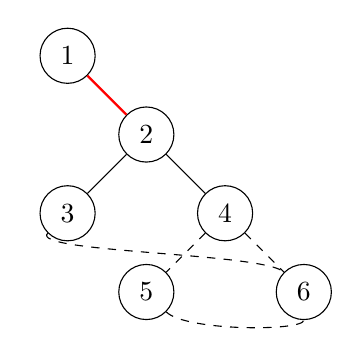
\begin{tikzpicture}[every node/.style={circle, draw, minimum size=0.7cm, inner sep=0pt}]
    \node (1) at (0,2) {1};
    \node (2) at (1,1) {2};
    \node (3) at (0,0) {3};
    \node (4) at (2,0) {4};
    \node (5) at (1,-1) {5};
    \node (6) at (3,-1) {6};

    \draw[red, thick] (1) -- (2);
    \draw (2) -- (3);
    \draw (2) -- (4);
    \draw[dashed] (4) -- (5);
    \draw[dashed] (4) -- (6);
    \draw[dashed] (3) .. controls (-0.5,-0.5) and (2.5,-0.5) .. (6); % thêm cạnh (3,6)
    \draw[dashed] (5) .. controls (1.5,-1.5) and (3,-1.5) .. (6); % thêm cạnh (5,6)
\end{tikzpicture}
\end{center}

Tuy nhiên, có một trường hợp cần chú ý: cạnh thêm vào có thể đã có sẵn trong đồ thị. Khi đó, ta cần tìm cạnh cầu trong một đa đồ thị, ta sẽ phải đánh dấu nếu cạnh đó đã sử dụng. \\

Để đánh dấu, ta có thể nén $id(u, v) = \min(u, v) \times 2\mathrm{e}5 + \max(u, v)$, lưu vào hashmap để truy vấn kiểm tra nhanh (tạm gọi là \texttt{edge\_cnt}). Sau đó kiểm tra cầu của đồ thị, nếu $edge\_cnt[id(u, v)] == 1$ thì đó là cầu.

\paragraph{Cài đặt}
\begin{lstlisting}[language=C++]
#include <bits/stdc++.h>
#define int long long
#define endl "\n"
using namespace std;
const int MAXN = 2e5;
vector<int> adj[200005];
unordered_map<int, int> edge_cnt;
int n;
int low[MAXN + 5] = {0}, num[MAXN + 5] = {0};
int bridge = 0, timeDfs = 0;

int id(int a, int b) {
    return min(a, b) * MAXN + max(a,b);
}
void dfs(int u, int parent) {
    low[u] = num[u] = ++timeDfs;

    for (auto v : adj[u]) {
        if (v == parent) continue;
        if (num[v] == 0) {
            dfs(v, u);
            low[u] = min(low[v], low[u]);
            int a = u, b = v;
            if (low[v] > num[u] && edge_cnt[id(a,b)] == 1) {
                bridge++;
            }
        }
        else {
            low[u] = min(low[u], num[v]);
        }
    }
}
signed main() {
    ios_base::sync_with_stdio(0);
    cin.tie(0);
    cout.tie(0);
    cin >> n;
    for (int i = 1; i < n; i++) {
        int u, v; cin >> u >> v;
        adj[u].push_back(v);
        adj[v].push_back(u);
        edge_cnt[id(u,v)]++;
    }
    int m; cin >> m;
    for (int i = 1; i <= m; i++) {
        int u, v; cin >> u >> v;
        adj[u].push_back(v);
        adj[v].push_back(u);
        if (u > v) swap(u, v);
        if (edge_cnt.find(id(u,v)) != edge_cnt.end()) edge_cnt[id(u,v)]++;
    }
    for (int i = 1; i <= n; i++) {
        if (num[i] == 0) {
            dfs(i,i);
        }
    }
    cout << bridge;
    return 0;
}
\end{lstlisting}



\section{Thành phần liên thông mạnh (Strongly Connected Components)}

\begin{dinhnghia}
    
\end{dinhnghia}
 
\begin{itemize}
    \item Một đồ thị có hướng là liên thông mạnh nếu như từ một đỉnh bất kì luôn tồn tại ít nhất một đường đi đến bất kì đỉnh nào khác.
    \item Một thành phần liên thông mạnh của một đồ thị có hướng là một đồ thị con tối đại liên thông mạnh. Nếu mỗi thành phần liên thông mạnh được co lại thành một đỉnh, thì đồ thị sẽ trở thành một đồ thị có hướng không có chu trình.
    \item Thuật toán \textit{Kosaraju}, thuật toán \textit{Tarjan}, và thuật toán \textit{Gabow} đều có thể tìm các thành phần liên thông mạnh của một đồ thị cho trước trong thời gian tuyến tính. Tuy nhiên, các thuật toán của \textit{Tarjan} thường được sử dụng nhiều hơn do chúng chỉ cần thực hiện tìm kiếm theo chiều sâu một lần trong khi thuật toán của \textit{Kosaraju} cần hai lần.
\end{itemize}

\begin{figure}[h]
    \centering
    \includegraphics[width=0.4\textwidth]{resource/img/b5/Depth-First-Search-Tree_img14.png}
    \caption{Minh họa thành phần liên thông mạnh (vùng xanh)}
\end{figure}

\subsection*{Một số định lý quan trọng}

\textbf{Định lý 1:} Nếu $a, b$ là hai đỉnh thuộc thành phần liên thông mạnh $C$ thì với mọi đường đi từ $a$ tới $b$ cũng như từ $b$ tới $a$, tất cả đỉnh trung gian trên đường đi đó đều phải thuộc $C$.

\textit{Chứng minh:} Nếu $a$ và $b$ là hai đỉnh thuộc $C$ thì tức là có một đường đi từ $a$ đến $b$ và một đường khác đi từ $b$ về $a$. Suy ra với một đỉnh $v$ nằm trên đường đi từ $a$ tới $b$ là ta tới được $v$, từ $b$ có đường tới $a$ nên $v$ cũng tới được $a$. Vậy $v$ nằm trong thành phần liên thông mạnh của $a$ tức là $v$ thuộc $C$. Trong tự vị mọi đỉnh nằm trên đường đi từ $b$ tới $a$.

\vspace{1em}
\textbf{Định lý 2:} Với một thành phần liên thông mạnh $C$ bất kỳ, tồn tại một đỉnh $r$ thuộc $C$ sao cho mọi đỉnh của $C$ đều thuộc cây con gốc $r$ trong cây \textit{DFS}.

\textit{Chứng minh:} Trước hết, nhắc lại một thành phần liên thông mạnh là một đồ thị con liên thông mạnh của đồ thị ban đầu thỏa mãn tính chất đại tại tức là không thể thêm một đỉnh nào vào mà vẫn giữ tính liên thông mạnh.\\
Trong số các đỉnh của $C$, chọn r là đỉnh được thăm đầu tiên khi thực hiện tìm kiếm theo chiều sâu. Ta sẽ chứng minh C nằm toàn bộ trong nhánh \textit{DFS} gốc $r$.\\
Thật vậy, với mọi đỉnh $v$ bất kỳ của $C$, có liên thông mạnh nên phải tồn tại một đường đi từ $r$ tới $v$: $(r = x_1, x_2, \dots, x_t = v)$.\\
Từ định lý 1, tất cả các đỉnh $x_1, x_2, \dots, x_t$ đều thuộc $C$ nên chúng sẽ phải thăm sau đỉnh $r$. Khi thủ tục \textit{DFS(r)} được gọi thì tất cả các đỉnh $x_1, x_2, \dots, x_t$ đều chưa thăm; như vậy thủ tục \textit{DFS(r)} sẽ liệt kê tất cả những đỉnh chưa thăm đến được từ r bằng cách xây dựng nhánh gốc r của cây \textit{DFS}, nên các đỉnh $x_1, x_2, \dots, x_t = v$ sẽ thuộc nhánh gốc r của cây \textit{DFS}. Bởi chọn r là đỉnh bất kỳ trong C nên ta có điều phải chứng minh.

Đỉnh $r$ trong chứng minh định lý - đỉnh thăm trước tất cả các đỉnh khác trong $C$ - gọi là chốt của thành phần C. Mỗi thành phần liên thông mạnh chỉ có một hoặc một vài chốt. Xét vị trí tương đối giữa các chốt trên cây \textit{DFS}, chốt của một thành phần liên thông mạnh là đỉnh nằm cao nhất so với các đỉnh khác thuộc thành phần đó, nói cách khác: là tiến đầu tiên để đi vào thành phần liên thông mạnh đó.

\vspace{1em}
\textbf{Định lý 3:} Luôn tìm được đỉnh chốt a thỏa mãn: Quá trình tìm kiếm theo chiều sâu bắt đầu từ a không thăm được bất kỳ một chốt nào khác. (Tức là nhánh \textit{DFS} gốc a không chứa một chốt nào nào ngoài a) chẳng hạn ta chọn a là chốt được thăm sau cùng trong một dãy chuyên về quy hoạch cho các chốt để thăm sau tất cả các chốt khác. Với chốt a như vậy thì các đỉnh thuộc nhánh \textit{DFS} gốc a chính là thành phần liên thông mạnh chứa a.

\textit{Chứng minh:} Với mọi đỉnh $v$ nằm trong nhánh \textit{DFS} gốc a, a là chốt của thành phần liên thông mạnh chứa v. Ta sẽ chứng minh bằng phản chứng. Nếu tồn tại một chốt $b \neq a$ phải nằm trong nhánh \textit{DFS} gốc a, thì nó sẽ mâu thuẫn với giả sử đã sắp xếp để a thăm sau các chốt khác. Vậy vẹn toàn trong nhánh \textit{DFS} gốc a và nhánh \textit{DFS} gốc a. Giả sử chứng rằng a khác b thì sẽ có hai trường hợp xảy ra.

\textbf{Trường hợp 1:} Nhánh \textit{DFS} gốc a chứa nhánh \textit{DFS} gốc b, có nghĩa là thủ tục \textit{DFS(b)} sẽ tới thủ tục \textit{DFS(a)} gọi tới, điều này mâu thuẫn với giả thiết rằng a là chốt mà quá trình tìm kiếm theo chiều sâu bắt đầu từ a không thăm một chốt nào khác.

\textbf{Trường hợp 2:} Nhánh \textit{DFS} gốc a và nhánh \textit{DFS} gốc b có nghĩa là a nằm trên một mớn đường từ b tới v. Do b và v thuộc cùng một thành phần liên thông mạnh nên theo định lý 1, a cũng phải thuộc thành phần liên thông mạnh đó. Suy ra b và a cùng là chốt của thành phần liên thông mạnh này có hai chốt a và b. Điều này vô lý.

Trong nhánh \textit{DFS} gốc a toàn thành phần liên thông mạnh chứa a, mà trong nhánh \textit{DFS} gốc a, theo chứng minh trên ta lại có: Mọi thành phần \textit{DFS} gốc a nằm trong thành phần liên thông mạnh chứa a. Kết hợp lại được: Nhánh \textit{DFS} gốc a chính là thành phần liên thông mạnh chứa a.

\begin{baitap}{Tìm TPLT mạnh}{https://oj.vnoi.info/problem/tjalg}

Cho đồ thị $G(V, E)$ có hướng $N$ $(1\leq N \leq 10^4)$ đỉnh $M$ $(1 \leq M \leq 10^5)$ cung. Hãy đếm số thành phần liên thông mạnh.\\

\textbf{Input}

Dòng đầu tiên là $M$, $N$.

$M$ dòng tiếp theo gồm 2 số nguyên $u, v$ mô tả một cung của $G$.\\

\textbf{Output} \\

Gồm một dòng duy nhất là số TPLT mạnh.\\

\textbf{Ví dụ}

\paragraph{Input}
\begin{lstlisting}
3 2
1 2
2 3
\end{lstlisting}

\paragraph{Output}
\begin{lstlisting}
3
\end{lstlisting}

\end{baitap}

\textbf{Thuật toán Tarjan}

\begin{figure}[h]
    \centering
    \includegraphics[width=0.6\textwidth]{resource/img/b5/Depth-First-Search-Tree_img15.png}
\end{figure}

\textbf{Thuật toán Tarjan được xây dựng dựa trên các dữ kiện sau:}
\begin{itemize}
    \item Tìm kiếm \textit{DFS} tạo ra cây/rừng \textit{DFS}.
    \item Các thành phần liên thông mạnh tạo thành các cây con của cây \textit{DFS}.
    \item Nếu ta có thể tìm được đỉnh gốc của các cây con như vậy, ta có thể in/lưu trữ tất cả các nút trong cây con đó (bao gồm cả đỉnh gốc) và đó sẽ là một thành phần liên thông mạnh (\textit{Strongly Connected Components - SCC}).
    \item Không có cung ngược từ \textit{SCC} này sang \textit{SCC} khác (Có thể có các cung chéo, nhưng các cung chéo sẽ không được sử dụng trong khi xử lý đồ thị).
\end{itemize}

\textbf{Ý tưởng}
\begin{itemize}
    \item \textbf{Nhận xét:} Xét cây con gốc $u$ trong cây \textit{DFS}. Gọi tập hợp các đỉnh thuộc cây con gốc $u$ là $A$, tập hợp các đỉnh không thuộc cây con gốc $u$ là $B$. Nếu tồn tại 1 đỉnh $x$ thuộc $A$ tới được 1 đỉnh $y$ thuộc $B$ thì phải có thứ tự thăm sớm hơn $u$. Vì nếu $y$ được thăm sau $u$ ta có thể duyệt từ $u$ qua $x$ tới $y$ khi đó $y$ sẽ trở thành con của $u$.
    \item Đầu tiên ta thực hiện \textit{DFS} kết hợp tính mảng \texttt{low[]}, \texttt{num[]} như đã trình bày ở trên. Song song với việc này, khi duyệt tới đỉnh $u$ ta sẽ thực hiện đẩy $u$ vào \textit{stack}.
    \item Khi đã duyệt xong đỉnh $u$ (sau khi duyệt hết toàn bộ các đỉnh trong cây \textit{DFS} gốc $u$), nếu $num[u] = low[u]$ thì đây chính là đỉnh có thứ tự thăm sớm nhất của một thành phần liên thông mạnh.
    \item Khi đó ta sẽ loại bỏ tất cả các đỉnh trong thành phần liên thông mạnh này ra khỏi đồ thị và các đỉnh này là các đỉnh đang nằm trên $u$ trong \textit{stack} hiện tại vì các đỉnh này chính là các đỉnh nằm con gốc $u$ trong cây \textit{DFS} do các nút được đẩy vào \textit{stack} theo thứ tự thăm.
    \item Mặt khác, giả sử ta có đỉnh $x$ thuộc cây con gốc $u$ và $x$ thuộc thành phần liên thông mạnh không chứa $u$ có đỉnh có thứ tự thăm sớm nhất là $y$, để thấy $y$ phải là con của $u$ và nên thôi duyệt đỉnh $y$ sớm hơn $u$ chứng tỏ $y$ và thành phần liên thông mạnh chứa nó sẽ bị loại bỏ trước đó không còn trong \textit{stack} nữa (nếu còn thì ở đó vì ta đang xét mọi đỉnh trong cây con gốc $u$ chưa được xác định nằm trong thành phần liên thông mạnh nào trong các con gốc $u$).
    \item Ta sẽ đánh dấu tất cả các đỉnh thuộc thành phần liên thông mạnh bằng 1 mảng để sau này không xét lại đỉnh đấy nữa. Đồng thời, ta loại bỏ các đỉnh này ra khỏi \textit{stack} để không làm ảnh hưởng tới các đỉnh khác vẫn còn nằm trong đồ thị.
\end{itemize}

\subsection*{Cài đặt}

\textbf{Cấu trúc dữ liệu:}
\begin{itemize}
    \item Hằng số \texttt{maxN = 10000}
    \item Biến \texttt{timeDfs} -- Thứ tự \textit{DFS}
    \item Biến \texttt{scc} -- Số lượng thành phần liên thông mạnh
    \item Mảng \texttt{low[]}, \texttt{num[]}
    \item Mảng \texttt{deleted[]} -- Đánh dấu các đỉnh đã bị xóa
    \item Vector \texttt{adj[]} -- Danh sách cạnh kề của mỗi đỉnh
    \item Ngăn xếp \texttt{st} -- Lưu lại các đỉnh trong thành phần liên thông mạnh
\end{itemize}

\begin{lstlisting}[language=C++]
#include <bits/stdc++.h>
#define int long long
#define endl "\n"
using namespace std;
vector<int> adj[10005];
int n, m, timeDfs = 0;
const int MAXN = 1e4;
stack<int> st;
vector<bool> deleted(MAXN + 5, false);
vector<int> num(MAXN + 5, 0), low(MAXN + 5, 0);
int scc = 0;
void dfs(int u) {
    st.push(u);
    num[u] = low[u] = ++timeDfs;
    for (auto v : adj[u]) {
        if (num[v] == 0) {
            dfs(v);
            low[u] = min(low[u], low[v]);
        }
        else {
            if (deleted[v] == false) low[u] = min(low[u], num[v]);
        }
    }
    if (low[u] == num[u]) {
        int cur;
        scc++;
        do {
        cur = st.top();
        deleted[cur] = true;
        st.pop();
        } while (cur != u);
    }
}

signed main() {
    cin >> n >> m;
    for (int i = 1; i <= m; i++) {
        int u, v; cin >> u >> v;
        adj[u].push_back(v);
    }    
    for (int i = 1; i <= n; i++) {
        if (num[i] == 0) {
            dfs(i);
        }
    }
    cout << scc;
}
\end{lstlisting}

%---------------------------%
\begin{baitap}{Truyền tin}{https://oj.vnoi.info/problem/message}

Một lớp gồm $N$ học sinh, mỗi học sinh cho biết những bạn mà học sinh đó có thể liên lạc được (chú ý liên lạc này là liên lạc một chiều: $u$ có thể gửi tin tới $v$ nhưng $v$ thì chưa chắc đã có thể gửi tin tới $u$).

Thầy chủ nhiệm đang có một thông tin rất quan trọng cần thông báo tới tất cả các học sinh. Để tiết kiệm thời gian, thầy chỉ nhắn tin tới một số học sinh rồi sau đó nhờ các học sinh này nhắn lại cho tất cả các bạn mà các học sinh đó có thể liên lạc được, và cứ lần lượt như thế làm sao cho tất cả các học sinh trong lớp đều nhận được tin.

Hãy tìm một số ít nhất các học sinh mà thầy chủ nhiệm cần nhắn.

\textbf{Input}
\begin{itemize}
    \item Dòng đầu là $N, M$ ($N \leq 800$, $M$ là số lượng liên lạc 1 chiều)
    \item Một số dòng tiếp theo mỗi dòng gồm 2 số $u, v$ cho biết học sinh $u$ có thể gửi tin tới học sinh $v$
\end{itemize}

\textbf{Output} 
\begin{itemize}
    \item Gồm 1 dòng ghi số học sinh cần thầy nhắn tin.
\end{itemize}


\textbf{Ví dụ}

\paragraph{Input}
\begin{lstlisting}
12 15
1 3
3 6
6 1
6 8
8 12
12 9
9 6
2 4
4 5
5 2
4 6
7 10
10 11
11 7
10 9
\end{lstlisting}

\paragraph{Output}
\begin{lstlisting}
2
\end{lstlisting}

\end{baitap}

\textbf{Phân tích bài toán}

Đầu tiên, ta gom các đỉnh thành các \textbf{thành phần liên thông mạnh} (SCC) -- tức là xác định những nhóm đỉnh mà trong đó, bất kỳ bạn nào nhận được tin cũng có thể truyền tin cho tất cả các bạn còn lại trong cùng nhóm đó. Việc gom nhóm này giúp rút gọn bài toán: với mỗi SCC, chỉ cần một học sinh trong nhóm nhận tin thì cả nhóm sẽ nhận được tin.

Tiếp theo, ta xây dựng \textbf{đồ thị rút gọn} giữa các SCC: mỗi nhóm là một đỉnh, có cung nối từ nhóm này sang nhóm khác nếu có ít nhất một học sinh trong nhóm đầu liên lạc được với học sinh trong nhóm sau. Lúc này, tin chỉ có thể lan truyền từ SCC này sang SCC khác theo các cung của đồ thị rút gọn.

Bây giờ, chỉ cần xét \textbf{bậc vào} (\textit{in-degree}) của mỗi SCC trong đồ thị rút gọn:
\begin{itemize}
    \item Những nhóm nào có bậc vào lớn hơn 0 sẽ nhận được tin từ các nhóm khác.
    \item Ngược lại, các nhóm không có bậc vào (in-degree bằng 0) là những nhóm không nhận được tin từ bất kỳ nhóm nào khác. Vì vậy, thầy chủ nhiệm bắt buộc phải gửi tin trực tiếp cho ít nhất một học sinh ở mỗi nhóm này, để tin có thể lan truyền tiếp đi.
\end{itemize}

Tóm lại, đáp số là \textbf{số lượng SCC có bậc vào bằng 0} trong đồ thị rút gọn. Đây cũng chính là số học sinh ít nhất mà thầy cần nhắn tin ban đầu.

\begin{figure}[h]
    \centering
    \includegraphics[width=0.6\textwidth]{resource/img/b5/message.png}
    \caption{Đồ thị ban đầu và Đồ thị sau khi gom nhóm theo SCC}
\end{figure}

\paragraph{Cài đặt}
\begin{lstlisting}[language=C++]
#include <bits/stdc++.h>
#define int long long
#define endl "\n"
using namespace std;
vector<int> adj[805];
const int MAXN = 800;
int n, m, timeDfs = 0;
vector<int> num(MAXN + 5, 0), low(MAXN + 5, 0);
vector<bool> deleted(MAXN + 5, false);
stack<int> st;
int scc = 0;
vector<int> comp(MAXN + 5);

void dfs(int u) {
    st.push(u);
    num[u] = low[u] = ++timeDfs;
    for (auto v : adj[u]) {
        if (deleted[v]) continue;
        if (num[v] == 0) {
            dfs(v);
            low[u] = min(low[v], low[u]);
        }
        else {
            low[u] = min(low[u], num[v]);
        }
    }    
    if (num[u] == low[u]) {
        int cur;
        do {
            cur = st.top(); st.pop();
            deleted[cur] = true;
            comp[cur] = scc;
        } while (cur != u);
        scc++;
    }
}
signed main() {
    cin >> n >> m;
    for (int i = 1; i <= m; i++) {
        int u, v; cin >> u >> v;
        adj[u].push_back(v);
    }
    for (int i = 1; i <= n; i++) {
        if (num[i] == 0) dfs(i);
    }
    vector<int> in_deg(scc, 0);
    for (int u = 1; u <= n; u++) {
        for (auto v : adj[u]) {
            if (comp[u] != comp[v]) {
                in_deg[comp[v]]++;
            }
        }
    }
    int ans = 0;
    for (int i = 0; i < scc; i++) {
        if (in_deg[i] == 0) {
            ans++;
        }
    }
    cout << ans;
}
\end{lstlisting}

%---------------------------%
\begin{baitap}{VOI 06 Bài 5 - Mạng máy tính}{https://oj.vnoi.info/problem/nkonearc}

Một hệ thống $n$ máy tính (các máy tính được đánh số từ $1$ đến $n$) được nối lại thành một mạng bởi $m$ kênh nối, mỗi kênh nối hai máy nào đó và cho phép ta truyền tin một chiều từ máy này đến máy kia. Giả sử $s$ và $t$ là 2 máy tính trong mạng. Ta gọi đường truyền từ máy $s$ đến máy $t$ là một dãy các máy tính và các kênh nối chúng có dạng:
\[
s = u_1, e_1, u_2, \ldots, u_i, e_i, u_{i+1}, \ldots, u_{k-1}, e_{k-1}, u_k = t
\]
trong đó $u_1, u_2, \ldots, u_k$ là các máy tính trong mạng, $e_i$ là kênh truyền tin từ máy $u_i$ đến máy $u_{i+1}$ ($i = 1, 2, \ldots, k-1$).

Mạng máy tính được gọi là \textbf{thông suốt} nếu như đối với hai máy $u, v$ bất kỳ ta luôn có đường truyền tin từ $u$ đến $v$ và đường truyền tin từ $v$ đến $u$. Mạng máy tính được gọi là \textbf{hầu như thông suốt} nếu đối với hai máy $u, v$ bất kỳ, hoặc là có đường truyền từ $u$ đến $v$, hoặc là có đường truyền từ $v$ đến $u$.

Biết rằng mạng máy tính đã cho là hầu như thông suốt nhưng không thông suốt.

Yêu cầu: hãy xác định xem có thể bổ sung đúng một kênh truyền tin để biến mạng đã cho trở thành thông suốt được không?

\textbf{Input}
\begin{itemize}
    \item Dòng đầu tiên ghi 2 số nguyên $n$ và $m$.
    \item Dòng thứ $i$ trong số $m$ dòng tiếp theo mô tả kênh nối thứ $i$ bao gồm 2 số nguyên dương $u_i$ và $v_i$ cho biết kênh nối thứ $i$ cho phép truyền tin từ máy $u_i$ đến máy $v_i$, $i = 1, 2, \ldots, m$.
\end{itemize}
Các số trên cùng một dòng được ghi cách nhau bởi dấu cách.

\textbf{Output}
\begin{itemize}
    \item Dòng đầu tiên ghi 'YES' nếu câu trả lời là khẳng định, ghi 'NO' nếu câu trả lời là phủ định.
    \item Nếu câu trả lời là khẳng định thì ghi ra hai số nguyên dương $u, v$ cách nhau bởi dấu cách cho biết cần bổ sung kênh truyền tin từ máy $u$ đến máy $v$ để biến mạng thành thông suốt.
\end{itemize}

\textbf{Giới hạn}

Trong tất cả các test, $n \leq 2000, m \leq 30000$.

\textbf{Ví dụ}

\paragraph{Input}
\begin{lstlisting}
3 2
1 2
2 3
\end{lstlisting}

\paragraph{Output}
\begin{lstlisting}
YES
3 1
\end{lstlisting}

\textbf{Minh họa ví dụ, cạnh đỏ là cạnh cần thêm vào để đồ thị thông suốt}

\begin{center}
    \begin{tikzpicture}[every node/.style={circle,draw,minimum size=1cm,inner sep=0pt}, 
        >=Stealth, node distance=2.2cm]
        % Các đỉnh
        \node (1) at (0,0) {1};
        \node (2) at (1.5,2) {2};
        \node (3) at (3,0) {3};

        % Các cạnh gốc
        \draw[->, thick] (1) -- (2);
        \draw[->, thick] (2) -- (3);

        % Cạnh thêm (đỏ)
        \draw[->, thick, red] (3) to [bend left=20] (1);
    \end{tikzpicture}
\end{center}

\end{baitap}

\textbf{Phân tích bài toán}

Đầu tiên, ta gom các đỉnh của đồ thị gốc thành các SCC. Kết quả thu được là một đồ thị rút gọn, trong đó mỗi SCC được coi là một siêu-đỉnh. Bài toán bổ sung đúng một cạnh để đồ thị trở thành liên thông mạnh tương đương với việc bổ sung một cạnh vào đồ thị rút gọn sao cho toàn bộ các SCC hợp thành một chu trình duy nhất.

Để làm được điều này, ta nhận thấy: trong đồ thị rút gọn, một siêu-đỉnh $u$ là ứng viên đầu nối nếu nó có bậc ra bằng 0 (deg\_out$[u]=0$) và bậc vào lớn hơn 0 (deg\_in$[u] > 0$); ngược lại, một siêu-đỉnh $v$ là ứng viên đuôi nối nếu nó có bậc vào bằng 0 (deg\_in$[v]=0$) và bậc ra lớn hơn 0 (deg\_out$[v] > 0$).

Khi đó, chỉ cần nối một cạnh từ một siêu-đỉnh thuộc đồ thị rút gọn có bậc ra bằng 0 đến một siêu-đỉnh thuộc đồ thị rút gọn có bậc vào bằng 0 là đủ để biến đồ thị thành liên thông mạnh.

%\begin{multicols}{2}

\paragraph{Cài đặt}
\begin{lstlisting}[language=C++]
#include <bits/stdc++.h>
#define int long long
#define endl "\n"
using namespace std;
vector<int> adj[2005];
const int MAXN = 2000;
int n, m, timeDfs = 0;
stack<int> st;
vector<bool> deleted(MAXN + 5, false);
vector<int> deg_in(MAXN + 5, 0), deg_out(MAXN + 5, 0);
vector<int> num(MAXN + 5, 0), low(MAXN + 5, 0);
vector<int> comp(MAXN + 5, 0);
int scc = 0;

void dfs(int u) {
    num[u] = low[u] = ++timeDfs;
    st.push(u);
    for (auto v : adj[u]) {
        if (deleted[v] == true) continue;
        if (num[v] == 0) {
            dfs(v);
            low[u] = min(low[u], low[v]);
        }
        else {
            low[u] = min(low[u], num[v]);
        }
    }

    if (low[u] == num[u]) {
        int v;
        do {
            v = st.top(); st.pop();
            deleted[v] = true;
            comp[v] = scc;
        } while (v != u);
        scc++;
    }
}
signed main() {
    cin >> n >> m;
    for (int i = 1; i <= m; i++) {
        int u, v; cin >> u >> v;
        adj[u].push_back(v);
    }
    for (int i = 1; i <= n; i++) {
        if (num[i] == 0) dfs(i);
    }
    for (int u = 1; u <= n; u++) {
        for (auto v : adj[u]) {
            if (comp[u] != comp[v]) {
                deg_out[comp[u]]++;
                deg_in[comp[v]]++;
            }
        }
    }

    int u = -1, v = -1;
    for (int i = 0; i < scc; i++) {
        if (deg_out[i] == 0 && deg_in[i] > 0) {
            if (u != -1) {
                cout << "NO";
                return 0;
            }
            u = i;
        }
        if (deg_in[i] == 0 && deg_out[i] > 0) {
            if (v != -1) {
                cout << "NO";
                return 0;
            }
            v = i;
        }
    }
    bool ok1 = false, ok2 = false;
    for (int i = 1; i <= n; i++) {
        if (comp[i] == u && ok1 == false) {
            u = i;
            ok1 = true;
        }
        if (comp[i] == v && ok2 == false) {
            v = i;
            ok2 = true;
        }
    }
    cout << "YES\n" << u << " " << v;
}
\end{lstlisting}
%\end{multicols}


%---------------------------%
\begin{baitap}{Coin Collector}{https://cses.fi/problemset/task/1686}

Một trò chơi gồm $n$ căn phòng và $m$ đường hầm nối giữa chúng. Mỗi phòng có một số lượng xu nhất định. Hỏi số lượng xu lớn nhất bạn có thể thu thập được khi di chuyển qua các đường hầm, trong trường hợp bạn được phép tự do chọn phòng bắt đầu và phòng kết thúc?

\textbf{Input}
\begin{itemize}
    \item Dòng đầu tiên gồm hai số nguyên $n$ và $m$: số lượng phòng và số lượng đường hầm. Các phòng được đánh số từ $1, 2, \ldots, n$.
    \item Dòng tiếp theo gồm $n$ số nguyên $k_1, k_2, \ldots, k_n$: số lượng xu ở mỗi phòng.
    \item Cuối cùng là $m$ dòng mô tả các đường hầm. Mỗi dòng gồm hai số nguyên $a$ và $b$, nghĩa là có một đường hầm một chiều từ phòng $a$ tới phòng $b$.
\end{itemize}

\textbf{Output}
\begin{itemize}
    \item In ra một số nguyên: số lượng xu lớn nhất bạn có thể thu thập được.
\end{itemize}

\textbf{Ràng buộc}
\begin{itemize}
    \item $1 \leq n \leq 10^5$
    \item $1 \leq m \leq 2 \cdot 10^5$
    \item $1 \leq k_i \leq 10^9$
    \item $1 \leq a, b \leq n$
\end{itemize}

\textbf{Ví dụ}

\paragraph{Input}
\begin{lstlisting}
4 4
4 5 2 7
1 2
2 1
1 3
2 4
\end{lstlisting}

\paragraph{Output}
\begin{lstlisting}
16
\end{lstlisting}

\end{baitap}

\textbf{Phân tích bài toán.}

Đầu tiên, ta gom các đỉnh của đồ thị gốc thành các SCC. Kết quả thu được là một đồ thị rút gọn, trong đó mỗi SCC được coi là một siêu-đỉnh, và giữa hai siêu-đỉnh $u$ và $v$ có cung hướng nếu tồn tại ít nhất một cạnh hướng từ một đỉnh trong SCC tương ứng với $u$ sang một đỉnh trong SCC tương ứng với $v$.  

Mỗi siêu-đỉnh $u$ mang trọng số bằng tổng số xu ở tất cả các phòng thuộc SCC đó. Do đồ thị rút gọn luôn là một đồ thị có hướng không chu trình (DAG), bài toán thu gọn thành việc tìm đường đi có tổng trọng số lớn nhất trên DAG này.

Gọi $\mathrm{dp}[u]$ là số xu lớn nhất có thể thu thập được khi xuất phát từ siêu-đỉnh $u$. Ta khởi tạo
\[
\mathrm{dp}[u] \;=\; \text{cost}[u],
\]
với \texttt{cost[u]} là trọng số (tổng xu) của SCC tương ứng. Sau đó, duyệt các cung $u \to v$ trên DAG (Code bên dưới thực hiện đệ quy có nhớ, có thể tối ưu hơn (hoặc không) bằng sắp xếp tô-pô), ta cập nhật
\[
\mathrm{dp}[u] \;=\; \max\bigl(\mathrm{dp}[u],\;\text{cost}[u] + \mathrm{dp}[v]\bigr).
\]
Cuối cùng, đáp án là
\[
\max_{u}\,\mathrm{dp}[u],
\]
tức tổng xu lớn nhất có thể thu thập khi được phép chọn tự do phòng bắt đầu (tương đương siêu-đỉnh $u$ khởi hành).  

\paragraph{Cài đặt}
\begin{lstlisting}[language=C++]
#include <bits/stdc++.h>
#define int long long
#define endl "\n"
using namespace std;
int n, m, timeDfs = 0, scc = 0;
const int MAXN = 1e5;
vector<int> k, adj[100005], num(MAXN + 5, 0), low(MAXN + 5, 0), comp(MAXN + 5, 0);
vector<bool> deleted(MAXN + 5, false);
vector<int> cost(MAXN + 5, 0), dp;
vector<vector<int>> bigNode;
stack<int> st;
void dfs(int u) {
    st.push(u);
    num[u] = low[u] = ++timeDfs;
    for (auto v : adj[u]) {
        if (deleted[v] == true) continue;
        if (num[v] == 0) {
            dfs(v);
            low[u] = min(low[u], low[v]);
        } else {
            low[u] = min(low[u], num[v]);
        }
    }
    if (num[u] == low[u]) {
        int v;
        do {
            v = st.top(); st.pop();
            deleted[v] = true;
            comp[v] = scc;
            cost[scc] += k[v];
        } while (v != u);
        scc++;
    }
}

void findCost(int u) {
    if (dp[u] != -1) return;
    dp[u] = cost[u];
    for (auto v : bigNode[u]) {
        findCost(v);
        dp[u] = max(dp[u], dp[v] + cost[u]);
    }
}

signed main() {
    cin >> n >> m;
    k.resize(n + 1);
    for (int i = 1; i <= n; i++) {
        cin >> k[i];
    }
    for (int i = 1; i <= m; i++) {
        int u, v; cin >> u >> v;
        adj[u].push_back(v);
    }
    for (int i = 1; i <= n; i++) {
        if (num[i] == 0) dfs(i);
    }
    bigNode.resize(scc);
    dp.resize(scc, -1);
    for (int u = 1; u <= n; u++) {
        for (auto v : adj[u]) {
            if (comp[u] != comp[v]) {
                bigNode[comp[u]].push_back(comp[v]);
            }
        }
    }
    for (int i = 0; i < scc; i++) {
        if (dp[i] == -1) {
            findCost(i);
        }
    }
    cout << *max_element(dp.begin(), dp.end());   
}
\end{lstlisting}

